\chapter{VERIFICATION ENVIRONMENT}
\label{chap:verification.tex}

\section {FUNCTIONAL VERIFICATION}

In SoC design methodology, the first step is to define the specifications. Once the system specifications are completed, design phase starts. The behavioral modeling of the design is done using hardware description languages like VHDL or Verilog HDL and in this stage the design is said to be Register Transfer Level aka RTL. It is then verified against functional requirements.  The verified RTL model is them mapped into an architecture made up of intellectual properties (IP) blocks. The system level verification is done to verify the architecture against the intended functional and other requirements. 



Functional verification validates that the design meets the requirements. Test cases are created based on the specifications. Various aspects of data and control flow are verified by passing information between external environments, communication with I/O devices,  software interactions etc. [ieee]

 
\section {TEST}

Most of the verification at AMD is for verifying the x-86 processor cores and SoC level IPs. At this level of abstraction, verification of interaction between the IPs and functional verification of top level modules are done.  Test conditions are written in x-86 assembly and in some cases written in high level languages like C++. The intension of each test is to verify specific functionality of the design and ensure its validity. The test plans must to be in sync with the specifications of RTL design and are to be updated with new specification changes to ensure that it is efficient enough to deal with all possible corner cases and boundary conditions. \\ Tests are developed so as to provide specific stimulus to the design and the outcome is compared aganist desired values to ensure validity. Ideally the design should be varified against all possible senarios that could arise and once it pass all the test it can be considered fully valid design. In cases where a particular test fails, the verification engineer needs to find out the cause of failure, understand the design or verification aspect that led to the particular situation and make appropriate changes. This is called debug step in verification. 

There are many possible issues that can lead to a test failure. Each test defines conditions for pass and fail. A fail or pass is basically the outcome of a test run. There can be manly different causes for test but most test failures are due to:    

\begin{itemize}
	\item[-] Self check 
	\item[-] Assertions/Checkers
\end{itemize}

A self check failure is caused due to self-tests. These are tests written such that they evaluate the results, compare it with desired value and finally report fail or pass. 

Assertions or checkers generally monitor particular signal or state during the design and report failure when ever the monitored value deviates from desired value. 

In this project we are considering self-test based verification and debugging of self-test failure.

%\subsection {DEVELOP TESTS}
%
%Tests for verifying all the features of the RTL are written in x86 assembly or in high level languages. These test plans are in sync with the specifications of RTL and are to be updated with new specification changes. Test cases should be efficient enough to deal with all possible []: 
%\begin{itemize}
%
%\item Corner cases
%\item Boundary conditions
%\item Design discontinuities
%\item Error conditions
%\item Exception/Interrupt handling
%
%\end {itemize}

\subsection {SELF TEST FAILURE}

Self-tests are test scenarios written to prove that device under test are functioning correctly in a specific situation. These are call "Self-test" as they are capable of deciding if the outcome was successful or not after simulation. These tests are normally hand written by the verification engineer rather than randomly generated.  Hence self-test can string together specific stimulus of interest and determine pass or fail status on its own without relying on another tool. \\

%\figurename{} 
\begin{figure}[H]
\centering
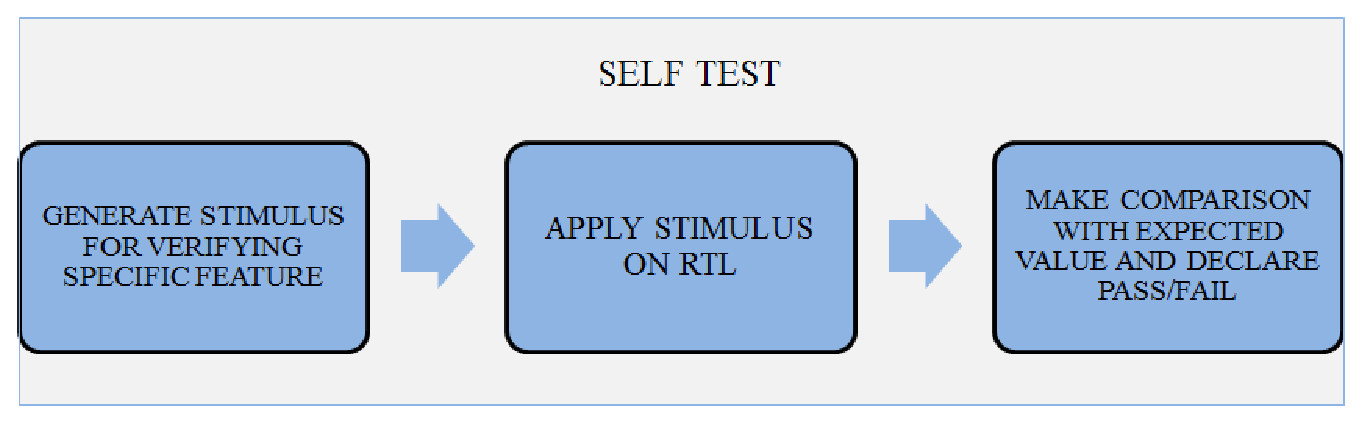
\includegraphics[width=5.5in]{./figures/selftest.ps}
\caption{Self-Test} 
\label{fig:selftest.ps}
\end{figure}

Figure x details the flow of a self test. In AMD most of the self-tests are a collection of x86 assembly language program. Tests are compiled by a script which calls an assembler producing an output that can be run on the RTL model. The stimuli are generated by the test and are applied to the DUT. The comparisons are done by the test itself and pass or fail flag is generated. \\



\section{DEBUGGING A SELF TEST FAILURE}

Self-tests report the occurrence of test case failure. Once this happens, next step is analyzing the reason for failure.  For this, a traceback from the point of failure to the point of error is required. 

A failure message indicates that the result is deviating from the desired value. This desired value can be understood from analysing the asm test code. But to understand at which point during execution the design deviated from the desired course, all the information regarding the execution flow as well as a reference flow which has the ideal values and status are required.
 
For this purpose of analyzing, the RTL is simulated along with an instruction level reference simulator. The reference simulator is a software model which imitates the design functionally and the runs in parallel with the RTL. This parallel simulation is known as co-simulation. 


\subsection {CO-SIMULATION}
The instruction level reference simulator aka ILS is an x86/x86-64 programming model. It mainly models the register states and memory features and act as the ideal reference point to compare with. The test provide stimulus to both the RTL model and reference model, the model will act as the ideal reference point. An interface between RTL and reference model compares the states after each instruction retire and report any mismatch. 

The following section details the features and functions of simulator and interface. 



%\figurename{} 
\begin{figure}[H]
\centering
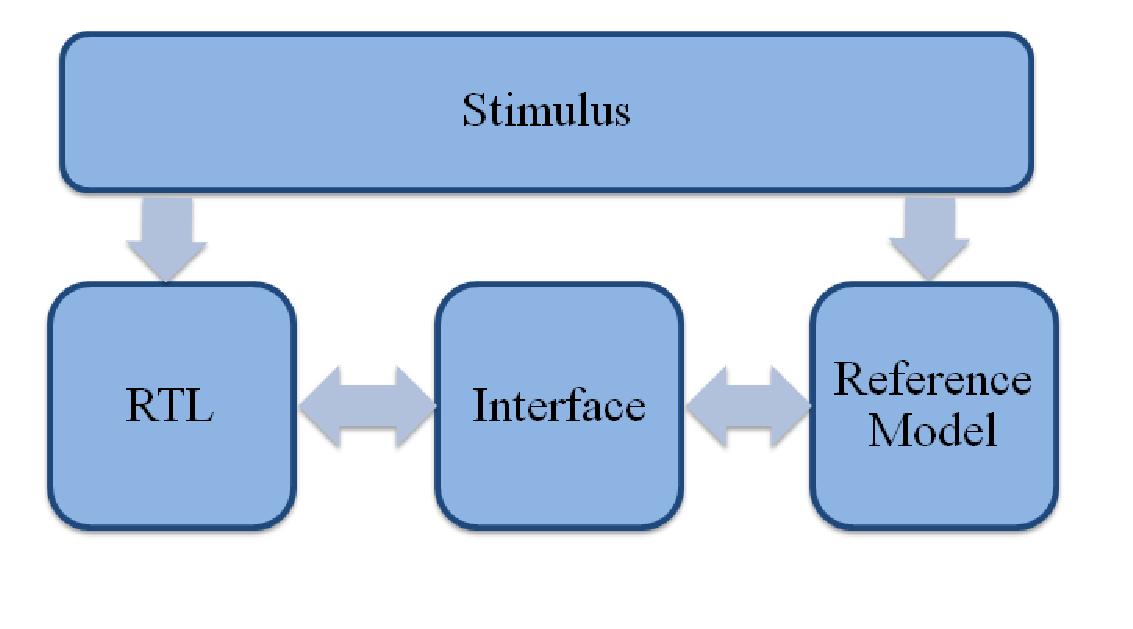
\includegraphics[width=4.5in]{./figures/interface.eps}
\caption{RTL-Reference Model Cosimulation} 
\label{fig:interface.eps}
\end{figure}



%\subsection {COMPARISON WITH REFERENCE MODULE}

%The RTL is simulated along with an instruction level reference simulator. This instruction level simulator is an x86/x86-64 programming model. It mainly models the register states and memory features and act as the ideal reference point to compare with. An interface between RTL and reference model compares the states after each instruction retire and report any mismatch. The following section details the features and functions of simulator and interface.

\subsubsection {INSTRUCTION LEVEL SIMULATOR}
The x86 instruction level simulator starts simulation with first initializing the contents of its memory from input files. The simulator emulates the fetch/decode/execute algorithm of a scalar processor, producing an output log known as processor execution log, describing the instruction, its results and any side effects on the processor state. The simulator models debug features, exceptions and interrupts as wellas processor specific features. Supported processor states include x86 general purpose registers, flag registers, control registers, media registers and most common model specific registers and both memory and I/O space. The simulator runs multi-threaded code to simulate multi-processor and multi-core processor systems. 
The simulator runs in step with the RTL. Whenever an instruction or exception is retired in RTL that thread within the simulator is stepped-up and the processor states in the RTL and simulator are compared. Difference detected in processor states are considered as mismatches; difference in memory locations written are considered as write mismatches and once these are found the co-simulation terminates. At the end of the simulation when all threads stop executing, the memory states of RTL and the simulator are compared and any discrepancies are reported as memory mismatches.

\subsubsection {INTERFACE}
The interface between RTL and reference model keeps the ILS in step with RTL signal. It steps the ILS after every instruction of the RTL has retired, and then compares the results of execution between RTL and ILs. If the reference model is unable to model anything that is present in the RTL, the interface also re-synchronizes the ILS with the state obtained after execution of the RTL instruction.
Main functions of this interface include [] :
\begin{itemize}
	\item Initialization: Initialize memory model, attach RTL signal and initial some specific RTL signals.
	\item Increment: Based on number of instruction retired per cycle, the interface informs ILS how many instructions to step.
	\item Interrupt Handling: Interface informs simulator about pending interrupts
	\item Comparing: Compares RTL and reference model registers; integer, FP, control and status word. Also reports any write mismatches. 
	\item Interfacing with the memory model: Tell memory model what operations are seen by the RTL. 
\end{itemize}


During the course of simulation, the ILS generates log files holding all the execution details. These are called "\emph {processor execution log}". These log files will contain cycle by cycle information regarding register states, memory values, flags, threads etc. Basically all the comparison and debugging will require these information.\\

Once the self test report a failure, simulation terminates and debug phase starts. For figuring out the cause of failure, verification engineer need to trace through this processor execution log files. Mismatches with reference model values provide information regarding the cause of failure. \\

Tracing through the log files is done manually. Data obtained from instruction simulation log and the compiled test files needs to be analyzed and co-related for debugging. This is a very tedious effort consuming a lot of verification time. This is because of two main reasons:

\begin{enumerate}
	\item Relevant/required information is buried under a wealth of information, and
	\item Co-related information is spread across in different files
\end{enumerate}

As the design itself is very complex, these reasons makes manual tracing too time consuming. This will stretch the verification time and ultimately time-to-market.   


